\documentclass[11pt]{article}
\usepackage[margin=1in]{geometry}
\usepackage{tikz}\usetikzlibrary{arrows.meta,positioning}
\usepackage{graphicx,booktabs,amsmath,amssymb,amsthm,hyperref,enumitem,xcolor,array,longtable,multirow}
\hypersetup{colorlinks,linkcolor=blue!50!black,citecolor=blue!50!black,urlcolor=blue!50!black}
\setlist{itemsep=2pt,topsep=3pt}\emergencystretch=3em
\setlength{\parskip}{4pt}\setlength{\parindent}{0pt}
\newtheorem{prop}{Proposition}
\newtheorem{rem}{Remark}
\newcolumntype{L}[1]{>{\raggedright\arraybackslash}p{#1}}
\newcommand{\ldf}{\mathrm{LDF}}
\newcommand{\ac}{\mathrm{AC}}

\title{Pathwise Safe Reinforcement Learning under Non-Smooth Polyhedral Constraints: A Differentiable World-Model Approach for Power Distribution Networks}
\author{Mihir Khatri\thanks{Corresponding author: mihir.khatri24@spit.ac.in}\\ \small Sardar Patel Institute of Technology (SPIT), Mumbai, India\\[4pt]
Rajesh Kolluri\\ \small Indian Institute of Information Technology, Design and Manufacturing (IIITDM) Kancheepuram, Chennai, India}
\date{}
\begin{document}\maketitle

\begin{abstract}
Learning-based controllers for cyber-physical systems are routinely required to respect polyhedral operating limits, yet the operators that map an infeasible action back into the admissible set are non-smooth, and their effect on policy gradients is seldom analysed. We study this problem on a canonical instance, the IEEE 33-bus radial distribution feeder supplying an electric-vehicle (EV) charging hub, using real sessions from two sites of the ACN-Data corpus (Caltech and JPL). The contribution is an architecture with four components, each isolated in its own ablation. (i) A physics-informed residual world model $\hat s=F_{\rm base}+N_\theta$ that is calibrated with split-conformal and adaptive conformal inference (ACI); we show that a margin fixed at one load level attains only 0.15, 0.08 and 0.06 coverage at 1.0, 1.25 and 1.5 times the calibration load (target 0.95), that ACI restores nominal coverage, and that the required margin scales with the square of the load, which is the signature of the $I^2R$ term omitted by LinDistFlow. (ii) A headroom statistic, defined against a violation-free reference tuned on training days, which bounds what a causal policy can gain and, once the oracle is corrected, is 3.5 to 10.0\% at Caltech and 15.2 to 25.7\% at JPL under three tariffs. (iii) A verified differentiable twin of the rollout (agreement with the simulator to $10^{-16}$) in which we prove that uniform ray-scaling restoration is homogeneous of degree zero on binding rows, so that it annihilates the gradient along the action scale, and replace it by a Cimmino-averaged orthogonal projection together with an inclusive-boundary clamp. (iv) Pathwise policy learning with this construction converges in every one of twelve runs, improves the tuned reference by 4.6 to 4.9\% (random split) and 5.2 to 5.5\% (strict 2019 chronological split) at JPL with no AC violations, and by 1.0 to 1.9\% at Caltech. The grid-only residual reduces the rating-normalised branch margin by a factor of 3.5 to 9.8. A negative result on bidirectional vehicle-to-grid dispatch is reported in full.
\end{abstract}
\textbf{Keywords:} safe reinforcement learning; differentiable simulation; pathwise policy gradient; polyhedral constraints; orthogonal projection; conformal prediction; LinDistFlow; distribution networks; EV charging.

%% =====================================================================
\section{Introduction}
Safe reinforcement learning has been developed largely around two devices: a penalty or Lagrangian that enforces constraints in expectation, and a projection layer that enforces them at every step given a model of the system [15, 12, 10]. The second device is attractive for physical infrastructure because a single violation can be costly. It carries a subtlety that is rarely examined. A projection onto a polyhedral set $\{p:\,Gp\le h\}$ is piecewise linear and generally not injective, and every cheaper surrogate for it, such as rescaling the action until the tightest row is met, is non-smooth at the faces and corners of the set. When the controller is trained by differentiating through a simulator, the Jacobian of this operator decides which directions of the policy parameters receive any learning signal at all [28, 29].

This paper studies that interaction in full, on a physical system where ground truth is available. The instance is a hub of $K=54$ EV charging ports attached to the IEEE 33-bus radial feeder [8]. The controller selects the power of each port every 15 minutes, subject to voltage and thermal limits that are enforced through the linearised LinDistFlow model while the executed action is evaluated against the exact branch-flow solution [9]. We chose this setting because it exhibits, in a compact form, all the features that make safe learning difficult: a polyhedral feasible set that changes at every step, a model error that grows with operating point, a cost with kinks (clipping at full charge, a running maximum for the demand charge), and an exact simulator that lets every claim be verified.

The architecture we propose is not specific to power systems. It combines a physics-informed residual world model $F_{\rm base}+N_\theta$ whose tail error is calibrated by adaptive conformal inference, a Cimmino-averaged orthogonal projection [33, 34] unrolled inside a differentiable twin, and a residual policy parametrisation anchored at a tuned reference. Any cyber-physical system whose admissible actions form a polyhedron that depends on the state, and whose dynamics admit a trustworthy analytic base model, can instantiate the same three components. We state this as a design principle and demonstrate it on one feeder and two real sites, and we make no claim of empirical validity beyond them.

The study began from the premise that a critic-based safe agent would outperform a tuned heuristic. That premise did not survive contact with real sessions, and the investigation that followed produced the results reported here. We do not recount the intermediate experiments; the evidence we rely on is limited to runs that are reproducible from the released code.

\paragraph{Outline.} Section~\ref{sec:domain} fixes the domain and notation. Sections~\ref{sec:problem} to~\ref{sec:gap} state the problem, the contributions and the position relative to prior work. Sections~\ref{sec:method} to~\ref{sec:methods} give the methodology, the formal problem and the proposed methods, including two propositions on the non-smoothness of the restoration operator. Sections~\ref{sec:data} and~\ref{sec:setup} describe the data and the experimental protocol, and Section~\ref{sec:results} the results. Section~\ref{sec:disc} discusses limitations, and Section~\ref{sec:concl} concludes.

%% =====================================================================
\section{Domain and Background}\label{sec:domain}
\subsection{EV charging hubs on a distribution feeder}
A charging hub is a set of $K$ ports behind one or more buses of a distribution feeder. A session has an arrival time, a departure time, a requested energy and a rated charging power. The operating cost has three components: energy purchased at a time-varying price, a penalty on energy that remains undelivered at departure, and a demand charge proportional to the day's peak aggregate power. Charging power is bounded by the port rating and by the state of charge (SoC), since charge acceptance declines near capacity. Ports that share a lateral lower the downstream voltage and load the upstream branches, so the action space is coupled by the network even when each vehicle's own problem is simple.

\subsection{Network model}
The feeder is the balanced single-phase IEEE 33-bus system [8]. The exact branch-flow equations on a tree [9] relate the squared voltage magnitudes $v_i$ and the branch flows $(P_{ij},Q_{ij})$ through quadratic terms that include losses. Neglecting those terms gives the LinDistFlow approximation, in which $v$ and the branch apparent-power surrogates are affine in the nodal injections. We denote by $\ac$ the exact solution obtained by backward-forward sweep and by $\ldf$ the linearisation. Unbalance and three-phase coupling are outside the model.

\subsection{Safety layers and conformal prediction}
A safety layer maps a proposed action to a nearby feasible action, typically by a quadratic program [10, 11, 12]. If the feasible set is constructed from a model, the guarantee is no stronger than the model. Split-conformal prediction [20, 21, 22] converts a calibration sample of model errors into a quantile margin with finite-sample marginal coverage under exchangeability. Adaptive conformal inference [23] updates the working level online by a feedback rule and maintains long-run average coverage without exchangeability.

\subsection{Differentiable simulation and pathwise gradients}
When the environment is a composition of differentiable operations, the gradient of the episode cost with respect to policy parameters can be obtained by backpropagation through the rollout, giving an analytic (pathwise) policy gradient [26, 27]. Such estimators typically have lower variance than score-function estimators but become biased or uninformative in the presence of discontinuities and stiff dynamics [28, 29]. The present problem contains three sources of non-smoothness: the box and SoC clipping, the running maximum of the demand charge, and the polyhedral restoration operator that is the principal object of study.

%% =====================================================================
\section{Problem Statement}\label{sec:problem}
We consider real-time dispatch of a charging hub on a fixed feeder with exogenous arrivals. Three questions are posed.

\textbf{P1: calibration of the projection model.} The safety layer sees only the linearised network. How large must the margin be so that the exact network remains within limits, how does the required margin behave when the load departs from the calibration load, and what is the cost of using independent per-constraint margins when joint coverage is required?

\textbf{P2: what can be gained.} For a causal, violation-free policy, what is the largest improvement over the best heuristic tuned on the same training days? Without this quantity a relative improvement over a baseline has no scale.

\textbf{P3: which learning signal.} Where an improvement is possible, does a critic-based agent or a policy trained through a differentiable twin capture it, and which property of the twin's construction decides whether the gradient is informative?

%% =====================================================================
\section{Contributions}\label{sec:contrib}
\begin{enumerate}
\item \textbf{Calibrated joint-coverage margins} for projection-based dispatch: measurement of the failure of fixed split-conformal margins under load shift, an ACI remedy, a physical explanation of the required growth as the square of the load, and a comparison of global, row-wise, Bonferroni and rating-normalised margins in terms of joint coverage.
\item \textbf{Headroom-gated evaluation}: a definition of headroom against a train-tuned violation-free reference, applied to real days under three tariffs, together with a diagnosis of why a perfect-foresight linear programme is not a lower bound and a correction to it.
\item \textbf{A verified differentiable twin and an analysis of the restoration operator}: a proof that uniform ray scaling is homogeneous of degree zero on binding rows, a Cimmino-averaged orthogonal projection that restores a tangential gradient, and an inclusive-boundary clamp that removes a stationary point at the reference policy.
\item \textbf{Pathwise policy learning that converges}: in twelve of twelve runs, with improvement over the tuned reference of 4.6 to 5.5\% at JPL on two splits and zero AC violations.
\item \textbf{A physics-plus-residual world model for calibration}: the grid-only residual reduces the rating-normalised branch margin by 3.5 to 9.8 times, with measured consequences for dispatch cost.
\item \textbf{A documented negative result} on bidirectional vehicle-to-grid dispatch and on critic-based baselines, with the associated headroom measurements.
\item \textbf{A reproducible package}: pinned versions, tests, result files and checksums.
\end{enumerate}


%% =====================================================================
\section{Related Work}\label{sec:related}
\textbf{Reinforcement learning for EV charging.} Surveys of reinforcement learning for demand response report sizeable gains over baselines [37]. EV2Gym [1] supplies a vehicle-to-grid simulator with heuristic, model predictive control and learning baselines, but does not model the distribution network. ACN-Data and ACN-Sim [5, 6] provide real session logs and a scheduling simulator with infrastructure constraints. The closest approach to ours is the physics-informed TD3 variant of Orfanoudakis et al. [2], which backpropagates the actor loss through $K$-step rollouts of a known power-flow and SoC model on 34- and 123-bus feeders. Multi-agent Lagrangian methods enforce voltage limits in expectation [3], and a field comparison of home energy management found rule-based, predictive and tree-based controllers within 0.6\% of each other and a reinforcement learning agent 25\% worse [4].

\textbf{Safe reinforcement learning and projection layers.} Constrained Markov decision processes and their algorithms [14, 15] enforce constraints in expectation during training. Action-correction layers [12], predictive safety filters [13] and differentiable optimisation layers [10, 11] enforce them per step given a model. Residual policy learning [17, 18] places a learned correction on a hand-designed controller, which is the parametrisation we adopt.

\textbf{Conformal prediction in control.} Split-conformal prediction [20, 21, 22] and ACI [23] are well established. In control, ACI has been used to set switching thresholds for learned safety filters [24], and conformal forecast intervals have been embedded in stochastic predictive control of charging hubs [25].

\textbf{Differentiable simulation.} Pathwise gradients through simulators have been exploited for continuous control [26, 27, 30, 31], and their failure modes under stiffness and discontinuity are documented [28, 29]. Differentiable AC power flow has been developed for speed [32].

Table~\ref{tab:rel} summarises the comparison.

\begin{table}[h]\centering\footnotesize\setlength{\tabcolsep}{3pt}
\begin{tabular}{@{}L{3.0cm}L{2.6cm}L{2.7cm}L{2.6cm}L{3.0cm}@{}}\toprule
Work & Feeder constraints & Differentiable model & Calibrated margin & Reference baseline\\\midrule
EV2Gym [1] & none & no & no & heuristics, MPC\\
ACN-Sim [6] & infrastructure limits & no & no & scheduling rules\\
Orfanoudakis et al. [2] & voltage (34, 123 bus) & yes, $K$-step & no & TD3, SAC, PPO, MPC\\
Huang et al. [3] & voltage (33 bus), expected & no & no & MARL variants\\
Zapico et al. [25] & hub capacity & no & conformal forecast & stochastic MPC\\
\textbf{This work} & voltage and thermal, exact AC check & yes, full episode & ACI, joint, residual-shrunk & tuned violation-free, oracle\\\bottomrule
\end{tabular}\caption{Closest related work along the four properties on which the present study differs.}\label{tab:rel}\end{table}

\textbf{Projection methods.} Simultaneous (Cimmino-type) row projections converge to a point of the intersection of half-spaces when it is non-empty and avoid the overshoot of summed sequential steps [33, 34]. Their role as a differentiable layer in a learning loop has, to our knowledge, not been analysed.

%% =====================================================================
\section{Research Gap}\label{sec:gap}
\begin{enumerate}
\item \textbf{No scale for learning gains.} Reported improvements are relative to baselines whose tuning budget and violation rate are unstated, and we found no study that reports a perfect-foresight bound against a violation-free tuned reference on real sessions.
\item \textbf{Calibration of the linearised model under shift.} Safety layers use a linearised network, yet we found no study that measures the LinDistFlow-to-AC error of the projected action, calibrates it conformally, and examines coverage under load shift and over many constraints jointly. To the best of our knowledge, no prior study has done so.
\item \textbf{The restoration operator inside a differentiable loop.} Differentiable-model methods use a restoration or projection step, but the Jacobian of that step has not been analysed with respect to the directions of policy parameter space that it renders uninformative.
\item \textbf{Effect of a physics prior on the conformal margin.} Residual world models are normally judged by mean prediction error, whereas a conformal margin is governed by the tail, and the effect of a learned residual on the required margin has not been reported for this problem.
\end{enumerate}

%% =====================================================================
\section{Methodology}\label{sec:method}
The pipeline (Fig.~\ref{fig:pipeline}) has a policy that proposes per-port power, a safety layer that projects it onto $\{p:\,G_tp\le h_t\}$ built from LinDistFlow rows and conformal margins, and a simulator that executes the projected action against the exact network. Three studies are arranged around this loop: calibration of the margins (P1), measurement of headroom with a tuned reference and a perfect-foresight oracle (P2), and learning with a critic or through the twin (P3).
\begin{figure}[h]\centering
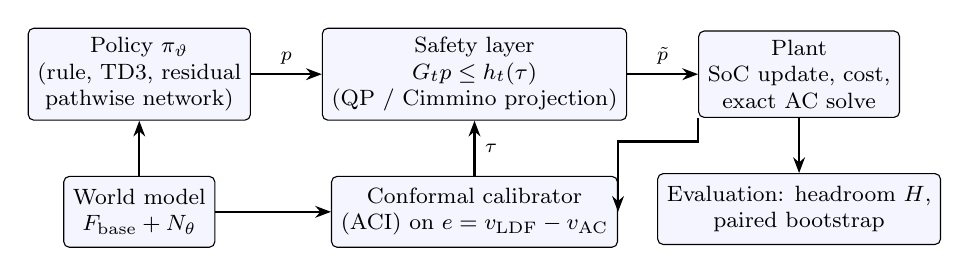
\begin{tikzpicture}[node distance=7mm and 9mm,box/.style={draw,rounded corners=2pt,minimum height=9mm,align=center,font=\footnotesize,fill=blue!4},arr/.style={-{Stealth[length=2mm]},thick}]
\node[box] (pol) {Policy $\pi_\vartheta$\\ (rule, TD3, residual\\ pathwise network)};
\node[box,right=of pol] (safe) {Safety layer\\ $G_tp\le h_t(\tau)$\\ (QP / Cimmino projection)};
\node[box,right=of safe] (plant) {Plant\\ SoC update, cost,\\ exact AC solve};
\node[box,below=of safe] (conf) {Conformal calibrator\\ (ACI) on $e=v_{\rm LDF}-v_{\rm AC}$};
\node[box,below=of pol] (wm) {World model\\ $F_{\rm base}+N_\theta$};
\node[box,below=of plant] (eval) {Evaluation: headroom $H$,\\ paired bootstrap};
\draw[arr] (pol)--node[above,font=\scriptsize]{$p$}(safe);
\draw[arr] (safe)--node[above,font=\scriptsize]{$\tilde p$}(plant);
\draw[arr] (plant)--(eval);
\draw[arr] (plant.south west)--++(0,-3mm)-|(conf.east) ;
\draw[arr] (conf)--node[right,font=\scriptsize]{$\tau$}(safe);
\draw[arr] (wm)--(conf);
\draw[arr] (wm.north)--(pol.south);
\end{tikzpicture}
\caption{Pipeline and evaluation loop.}\label{fig:pipeline}\end{figure}
Every comparison uses identical days, price, safety layer and cost function. References are tuned on training days only. Differences are paired by day with bootstrap intervals, and seeds are stated in each table. Training objectives are computed in the twin, but every reported cost is a simulator cost in which the action passes through the exact QP safety layer and the exact AC solver; this closed-loop protocol is the only one under which a restoration operator in the twin can be compared with the operator that is deployed.

%% =====================================================================
\section{Problem Formulation}\label{sec:form}
\textbf{Notation.} Time steps $t=1,\dots,T$ have length $\Delta t=0.25$ h. Synthetic days use $T=96$ (24 h). Real-session episodes use $T=192$ (48 h): arrivals occur in the first 24 h, and the second 24 h allows sessions that begin late in the day to dwell and depart after midnight, so that their energy accounting is closed inside the episode. Ports $k=1,\dots,K$. Occupancy $o_{k,t}\in\{0,1\}$, arrival, departure, rating $\bar p_{k,t}$, capacity $C_k$, initial SoC $s^0_k$ and target $s^{\rm tgt}_k$ are exogenous. Powers are in per unit of a base $S_b$.

\textbf{Dynamics.} For charging power $p_{k,t}\ge0$ and discharging power $q_{k,t}\ge0$,
\begin{equation}
s_{k,t+1}=\Pi_{[0,1]}\Big(s_{k,t}+\frac{\Delta t}{C_k}\big[\eta_c(s_{k,t})\,p_{k,t}-q_{k,t}/\eta_d(s_{k,t})\big]\Big),\qquad \eta_\bullet(s)=\eta_0-\kappa\,(s-\tfrac12)^2,
\end{equation}
with $\eta_0=0.95$ and $\kappa=0.22$. The unidirectional case sets $q\equiv0$. Power is bounded by $0\le p_{k,t}\le\bar p^{\,c}_{k,t}=\min\{\bar p_{k,t},(s_{\max}-s_{k,t})C_k/(\eta_0\Delta t)\}o_{k,t}$ and, when discharge is permitted, $0\le q_{k,t}\le\bar p^{\,d}_{k,t}=\min\{\bar p_{k,t},(s_{k,t}-s_{\min})C_k\eta_0/\Delta t\}o_{k,t}$.

\textbf{Network rows.} Let $x_t=p_t-q_t$ be the signed injection. In LinDistFlow, squared voltages and branch apparent-power surrogates are affine in $x_t$, so that the voltage limits $[0.95,1.05]$ p.u. and thermal limits, the latter represented by a polygon of cuts, take the form
\begin{equation}
G_t\,x_t\le h_t(\tau),\label{eq:poly}
\end{equation}
where $h_t$ contains the exogenous load, the ratings and the conformal margins $\tau$.

\textbf{Cost.}
\begin{equation}
J=\sum_t c_t\Delta t\,\mathbf 1^\top\!(p_t-\rho_s q_t)+\sum_{t,k}c_{\rm deg}(q_{k,t},s_{k,t})+\lambda_u\sum_k C_k\big(s^{\rm tgt}_k-s_{k,d_k}\big)_+ +\lambda_{\rm pk}\max_t \mathbf 1^\top x_t,
\end{equation}
with price $c_t$, sell ratio $\rho_s=0.92$, the degradation term $c_{\rm deg}=\beta (q S_b/10)^{1.35}\Delta t+\beta_{\rm dod}(1-s)^2\mathbf 1[q>0]$, unmet-energy penalty $\lambda_u=2$ \$/kWh and demand charge $\lambda_{\rm pk}$ in \$/kW-day.

\textbf{Control problem.} Find a causal policy $x_t=\pi(\mathcal I_t)$, with $\mathcal I_t$ the information available at $t$, minimising $\mathbb E[J]$ subject to \eqref{eq:poly} at every step and to the exact AC network remaining within limits.

\textbf{Calibration problem.} Let $e_t=\max_i(v^\ldf_{i,t}-v^\ac_{i,t})$ and $\sigma_t=\max_b(S^\ac_{b,t}-S^\ldf_{b,t})_+/\bar S_b$ be the one-sided voltage and rating-normalised flow errors. The margin $\tau$ is to satisfy $\Pr(\text{all exact-network limits hold at }t)\ge1-\alpha$.

\textbf{Headroom.} Let $J_{\rm ref}$ be the mean held-out cost of the best violation-free heuristic selected on training days and $J_{\rm LP}$ that of a perfect-foresight programme on the same network rows. Define
\begin{equation}
H=\frac{J_{\rm ref}-J_{\rm LP}}{J_{\rm ref}}.
\end{equation}
Within the model of the programme no causal violation-free policy can attain an expected gain exceeding $H$. The programme omits the SoC-dependent efficiency and is therefore not a bound on the simulator cost; Section~\ref{sec:res-head} quantifies the effect.

%% =====================================================================
\section{Proposed Methods}\label{sec:methods}
\subsection{Conformal margins under shift}
With score $s_t$ and target level $1-\alpha$, ACI maintains a working level $\alpha_{t+1}=\alpha_t+\gamma(\alpha-\mathbf 1[s_t>q_t])$ and sets the margin $q_t$ to the empirical $(1-\alpha_t)$ quantile of recent scores. For many constraints four margins are compared: a single global margin on branch apparent power; independent row-wise margins at level $\alpha$; Bonferroni margins at level $\alpha/m$ for $m$ rows; and the $(1-\alpha)$ quantile of the rating-normalised maximum $\max_b e_b/\bar S_b$. A load-normalised score $s_t/(g_t/g_{\rm nom})^{k}$, with $g_t$ the observable total load and $k$ fitted on the calibration set, is also evaluated.

\subsection{Tuned reference and perfect-foresight oracle}
The reference is the best of the projected full-rate rule and an earliest-deadline-first (EDF) policy under a site power cap swept over a grid, selected on training days under the condition that its mean violation after projection is zero. The oracle is a linear programme over the day with perfect knowledge of arrivals and prices, solved with the network rows of the safety layer. Its efficiency model is corrected as described in Section~\ref{sec:res-head}.

\subsection{Differentiable twin}
Because arrival and departure depend only on time, the day cost is, for fixed exogenous data, an almost-everywhere differentiable function of the action sequence. The rollout is implemented in double precision with the SoC recursion and its efficiency taper, energy cost, unmet-energy penalty at departure, demand charge as a running maximum, and the rows \eqref{eq:poly}. The exact AC solve is not part of the twin and is used only to evaluate executed actions. An action that violates \eqref{eq:poly} must be restored within the rollout.

\subsubsection{Restoration by ray scaling and its degeneracy}
Uniform ray scaling sets $\tilde p=\alpha(p)\,p$ with $\alpha(p)=\min\{1,\min_{i:(Gp)_i>0}h_i/(Gp)_i\}$.
\begin{prop}\label{prop:ray}
Let $h>0$ and suppose the minimum defining $\alpha(p)$ is attained at a row $i^\star$ with $(Gp)_{i^\star}>h_{i^\star}$, so that $\alpha(p)<1$. Then $\tilde p(cp)=\tilde p(p)$ for all $c>0$ in a neighbourhood of $1$, and consequently the Jacobian satisfies $\partial\tilde p/\partial p\cdot p=0$. For any differentiable loss $\mathcal L$, $\nabla_p\mathcal L(\tilde p(p))^\top p=0$.
\end{prop}
\begin{proof}
In a neighbourhood of $p$ the minimising row is unchanged, and $\alpha(cp)=h_{i^\star}/(c\,(Gp)_{i^\star})=\alpha(p)/c$. Hence $\tilde p(cp)=\alpha(cp)\,cp=\alpha(p)p=\tilde p(p)$. Differentiating $\tilde p(cp)$ with respect to $c$ at $c=1$ gives $(\partial\tilde p/\partial p)\,p=0$, and the chain rule gives the last claim.
\end{proof}
The overall scale of the proposed action is thus invisible to the cost whenever any row binds, so a policy that proposes full rate on every port is at a point where the gradient along the scale direction is exactly zero. Since in a congested hub rows bind for a large fraction of steps, the effect accumulates along the episode.

\subsubsection{Cimmino-averaged orthogonal projection}
Let $V_k=\{i:(Gp_k)_i>h_i\}$ be the violated rows. We apply, for $k=0,\dots,n-1$ with relaxation $\lambda\in(0,2)$,
\begin{equation}
p_{k+1}=\Pi_{[\underline p,\bar p]}\Big(p_k-\frac{\lambda}{\max(1,|V_k|)}\sum_{i\in V_k}\frac{(g_i^\top p_k-h_i)}{\|g_i\|^2+\varepsilon}\,g_i\Big),
\end{equation}
followed by a single ray scaling as a floating-point certificate of feasibility. The averaging weight $1/\max(1,|V_k|)$ is the Cimmino weighting [33, 34]. A summed step ($\lambda=0.5$ without averaging), which is what the standard Jacobi form gives, overshoots when many nearly parallel voltage rows are violated: on the starting rule the day cost rises from 1164 to 2443, whereas the averaged step gives 1140 (Section~\ref{sec:res-pgd}). If the iteration is stopped when a single row $g$ is active and $\lambda=1$, the Jacobian is $I-gg^\top/\|g\|^2$, whose null space is the normal $g$ and not the ray through $p$. The scale direction retains a gradient unless $p\parallel g$.

\subsubsection{Inclusive-boundary clamp}
A residual policy $u=\mathrm{clip}(u_{\rm base}+\beta\,\delta_\vartheta(x),0,1)$ with $\delta_\vartheta(x)\in[-1,1]$ starts at the reference when the output layer is zero. At the reference, $u_{\rm base}\in\{0,1\}$ lies on the boundary of the clip. The clamp of the common automatic-differentiation libraries assigns zero derivative exactly at the bounds.
\begin{prop}\label{prop:clip}
If the clip has zero derivative at its bounds and $\delta_\vartheta\equiv0$, then the gradient of the cost with respect to every parameter $\vartheta$ is zero at initialisation, for any differentiable downstream operator. Initialisation at the reference is therefore a stationary point of the surrogate.
\end{prop}
\begin{proof}
$\partial u/\partial\delta=\beta\,\mathbf 1[u_{\rm base}+\beta\delta\in(0,1)]$ equals $0$ at $\delta=0$ when $u_{\rm base}\in\{0,1\}$, and the chain rule propagates the zero.
\end{proof}
We replace the clip by a forward-exact version with derivative one on the closed interval,
$\mathrm{clip}_\iota(x)=\mathrm{sg}[\mathrm{clip}(x)]+(x-\mathrm{sg}[x])\,\mathbf 1[x\in[0,1]]$, with $\mathrm{sg}$ the stop-gradient. This preserves feasibility in the forward pass and gives the policy a usable direction at the reference.

\subsubsection{Policy and training}
The policy is a causal shared network applied to ten per-port features (price level and rank, SoC, deficit, remaining time, urgency, rating, site load, running peak) with a zero-initialised output layer, and is trained by Adam on the mean cost over training days, with a learning rate of $3\times10^{-3}$, gradient-norm clipping at 5, $\beta=0.5$, ten projection steps and no critic.

\subsection{Residual world model}
The model predicts the next voltage, branch flow and SoC as $\hat s_{t+1}=F_{\rm base}(s_t,a_t)+N_\theta(s_t,a_t)$, with $F_{\rm base}$ the LinDistFlow and SoC recursion. $N_\theta$ is a small network whose output is scaled to a few percent of the range of each variable and initialised near zero, trained on mean-squared error with a Kirchhoff-voltage-law penalty on the corrected prediction. Variants: $F_{\rm base}$ alone; $N_\theta$ with and without an SoC head; and a black-box network without the physics base. In the safety layer, the corrected voltage prediction of $N_\theta$ is used as an offset to the polytope and the calibrated margin of the chosen variant is applied.

\subsection{Critic-based baseline}
The critic-based comparator is the twin-delayed deep deterministic policy gradient algorithm (TD3) [16], with the QP layer placed after the actor and a residual structure around the tuned reference [17, 18]. Rewards are shaped by a potential function, which leaves the optimal policy unchanged [19]. An optional one-step model-based term, weighted by $\lambda_{\rm mb}$, adds to the actor loss the cost predicted by $F_{\rm base}+N_\theta$ for the next state, which tests a one-step horizon against the full-episode horizon of the pathwise method.

\subsection{Bidirectional extension}
For vehicle-to-grid dispatch the twin is extended with a signed action $u\in[-1,1]$, charge limit $\bar p^{\,c}$ for $u\ge0$ and the SoC-feasible discharge limit $\bar p^{\,d}$ for $u<0$, the two-way taper efficiency, and the degradation term above. The discomfort term of the simulator is omitted from the twin because the per-vehicle willingness weights are not part of the extracted day. The soft indicator $\tanh(qS_b/0.5)$ replaces $\mathbf 1[q>0]$ in the DoD term during training.

%% =====================================================================
\section{Dataset}\label{sec:data}
\textbf{Sessions.} The sessions are taken from ACN-Data [5], which provides the Caltech site (54 ports) and the JPL site (52 ports) for the period 2018 to 2021, each session being recorded with its connection and disconnection times and its delivered and requested energy. Only weekdays are used. Because the year 2020 is atypical, a strict chronological split within 2019 is evaluated in addition to a random split.

\textbf{Prices.} Four sources, each labelled in every table: (a) an SCE time-of-use stand-in schedule; (b) the SCE TOU-EV-4 schedule of March 2019 from the open-source \texttt{acnportal} package, applied to both sites and all years by assumption and including its demand charge; (c) the LBNL Wholesale Electricity Prices tool [7], hourly CAISO, a system-level series rather than a nodal price; (d) synthetic scenarios. A file of daily peak blocks was inspected and excluded for lack of hourly resolution.

\textbf{Feeder and load.} The feeder is the IEEE 33-bus system [8] with base power $S_b=1$ MVA, base voltage $V_b=12.66$ kV and its standard bus loads (3.715 MW and 2.3 Mvar in total). The ports are grouped into three hubs at the electrically deepest buses, 18, 17 and 16 of the standard numbering, which receive 51\%, 31\% and 18\% of the ports respectively. The chargers operate at unity power factor, so no reactive power is injected. Each branch thermal limit is represented by an inner octagon of eight linear cuts on $(P,Q)$, and branch ratings are 1.6 times the nominal base-load flow. The stress regime doubles EV load and limits hub capacity to two thirds of the site rating so that the network binds. Synthetic days come from a session generator with the same interface as the real loader.

\textbf{Splits.} Headroom: 20 evenly spaced weekdays per site. Random split: 50 evenly spaced weekdays, 30 for training and 20 for testing under a fixed seed. Chronological split: 30 weekdays from 1 January to 2 August 2019 for training and 20 from 9 August to 31 December 2019 for testing.

%% =====================================================================
\section{Experimental Setup}\label{sec:setup}
\textbf{Implementation.} The code is written in Python with PyTorch (double precision in the twin), NumPy, SciPy and CVXPY with the Clarabel and OSQP solvers. Library versions are pinned, and every experiment reported here was executed on CPU, where runs are bit-reproducible.

\textbf{Conformal experiments.} The margin is calibrated at $0.75$ times the nominal load ($n=2000$) and deployed on a load stream that ramps to $L\in\{1.0,1.25,1.5\}$ times nominal over 4000 steps. Twenty seeds are used with $\alpha=0.05$ and $\gamma=0.01$. Joint coverage is estimated on 2000 test scenarios for 32 branches at $\alpha=0.01$.

\textbf{Headroom.} Twenty weekdays per site are evaluated in the stress regime under three price sources. The candidate heuristics are EDF caps on a grid down to 0.1 of rating and the projected full-rate rule, and the oracle is the perfect-foresight linear programme solved through CVXPY.

\textbf{Pathwise learning.} Each configuration is trained for 150 Adam iterations with three seeds and evaluated on 20 held-out days in the simulator through the exact QP layer. No constraint violation is tolerated, and differences are summarised by a paired bootstrap with 4000 resamples, following the recommendations on seeds and interval estimates of [35, 36]. Evaluation under the training restoration is also recorded, which verifies that the twin and the simulator agree.

\textbf{Twin verification.} Identical random actions are passed through the twin and the simulator on 10 synthetic and 10 real days, and automatic differentiation is compared with central finite differences on 60 coordinates with non-zero gradient.

\textbf{World model.} Transitions are collected from the simulator under four rules (EDF caps of 1.0, 0.6 and 0.4, and the uncontrolled rule). The synthetic experiments use 30 training and 10 held-out days, and the real-data experiments use 16 training, 8 calibration and 10 test days per site, all disjoint. Margins at the 1\% level are calibrated on half of the calibration transitions and coverage is checked on the other half. The dispatch cost under each margin is then measured by running the tuned reference through the QP layer on the test days.

\textbf{Modular design of the ablations.} Each component is evaluated in isolation so that its effect is not confounded with the others. The pathwise experiments use the LinDistFlow rows with a fixed margin, the world-model experiments measure margins and the dispatch cost of the tuned reference, and the critic comparison fixes the data and the reference. A single end-to-end run in which the pathwise policy operates inside the residual-calibrated margin is left for future work.

\textbf{Vehicle-to-grid.} Eight synthetic days at normal load are used with the SCE stand-in price, an efficiency of 0.95 per direction with taper, degradation and the unmet-energy penalty, together with twenty held-out real days for the reference and oracle comparison. All costs are simulator costs.

\textbf{Critic baseline.} TD3 is trained for 120 episodes on freshly sampled synthetic stress days with three seeds and $\lambda_{\rm mb}\in\{0,0.5\}$.

%% =====================================================================
\section{Results}\label{sec:results}
\subsection{Safety margins under load shift}\label{sec:conf}
\textbf{Fixed margins fail.} A split-conformal margin calibrated at $0.75\times$ load covers 0.145, 0.081 and 0.064 of the deployment stream at $L=1.0,1.25,1.5$ (0.77, 0.62 and 0.51 over the first 500 steps) against a target of 0.95. ACI maintains 0.95 over the whole stream (Fig.~\ref{fig:conf}).
\begin{figure}[h]\centering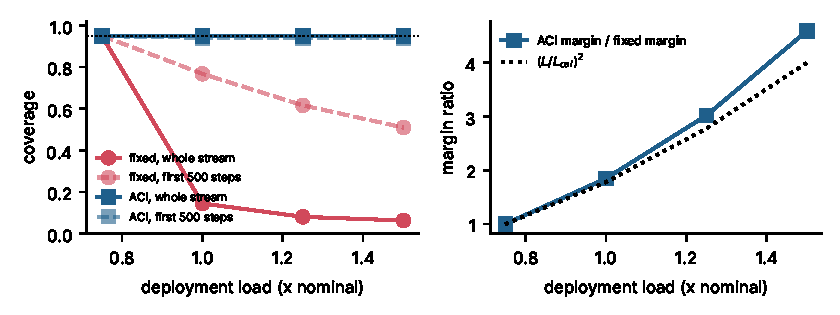
\includegraphics[width=.8\linewidth]{figs/fig_conformal_shift.pdf}\caption{Coverage under load shift (left; solid, whole stream; dashed, first 500 steps; dotted, target) and ACI margin relative to the fixed margin together with $(L/L_{\rm cal})^2$ (right).}\label{fig:conf}\end{figure}

\textbf{The required growth is physical.} The steady-state ACI margin is 1.85, 3.02 and 4.59 times the fixed one, against $(L/L_{\rm cal})^2=1.78,\,2.78,\,4.00$. To first order the LinDistFlow voltage error is the neglected loss term $\sum r_\ell\,(P_\ell^2+Q_\ell^2)/v_\ell$, which scales with the square of the branch current, so that a margin proportional to the square of the load is the expected outcome. A load-normalised score with fitted exponent $k=2.11$ restores fixed-margin coverage at $L=1.0$ (0.953) but not at 1.25 or 1.5 (0.667, 0.287); with ACI it lowers the margin by only 22 to 23\%. A scalar total load is an inadequate proxy for a quantity that depends on the spatial distribution of load, and a per-bus feature was not evaluated.

\textbf{Joint coverage requires a joint margin.} A single global margin on branch apparent power is 453 kVA at $\alpha=1\%$, exceeding 10\% of the rating on 30 of 32 branches and leaving weak branches without a safe set. Independent row-wise margins use at most 7.1\% of any rating and give per-branch coverage of at least 0.984, but a joint coverage of 0.932 against 0.99. Bonferroni margins restore 0.990 (at most 8.5\% of a rating, median 2.6\%), and a rating-normalised maximum score with one quantile gives 0.988 (7.1\% of every rating).

\subsection{Headroom on real days}\label{sec:res-head}
\textbf{A correction to the perfect-foresight programme.} Under the TOU-EV-4 tariff the programme returned the status \emph{optimal inaccurate} and a negative headroom. Two candidate causes were tested on eight JPL days. First, the discharge-degradation term enters the programme as a power atom with exponent 1.35, which CVXPY approximates by six second-order-cone constraints even when discharge is disabled. Removing it makes every solve \emph{optimal}, whereas tightening the solver tolerances to $10^{-10}$ or adding a strictly convex tie-breaker of $10^{-6}\sum p^2$ does not change the status. Second, the programme prices charging at a constant efficiency, whereas the simulator uses an SoC-dependent taper. The same plan costs 326.3 in the programme and 380.6 in the simulator, and the whole difference of 54.3 lies in the unmet-energy term. Derating the charging efficiency of the programme by $\kappa\,\mathbb E[(s-\tfrac12)^2]\approx0.013$ lowers the simulator cost of the executed plan from 381.6 to 349.9 and the gap between programme and simulator to 17 (Table~\ref{tab:lp}). The solver status was therefore not the cause of the negative headroom; the model mismatch was.
\begin{table}[h]\centering\small
\begin{tabular}{L{6.2cm}cc}\toprule Oracle variant (JPL, 8 days) & Programme cost & Simulator cost\\\midrule
Default (power cone, nominal efficiency) & 326.3 & 381.5\\
Tight tolerances & 326.3 & 381.5\\
Tie-breaker $10^{-6}$ & 326.3 & 381.0\\
No discharge atom, tie-breaker & 326.3 & 381.6\\
No discharge atom, tie-breaker, derated efficiency & 332.9 & 349.9\\
Projected full-rate reference & -- & 420.8\\\bottomrule
\end{tabular}\caption{Diagnosis of the oracle on eight JPL days under the TOU-EV-4 tariff. Status was \emph{optimal} on all days only when the discharge atom was removed.}\label{tab:lp}\end{table}

\textbf{Headroom.} Table~\ref{tab:head} reports $H$ with the corrected oracle.
\begin{table}[h]\centering\small
\begin{tabular}{L{4.4cm}cccccc}\toprule & \multicolumn{3}{c}{Caltech} & \multicolumn{3}{c}{JPL}\\ Price source & Ref. & LP & $H$ (\%) & Ref. & LP & $H$ (\%)\\\midrule
SCE time-of-use stand-in & 296.9 & 268.3 & 9.6 & 561.7 & 417.2 & 25.7\\
CAISO hourly (WEP) & 331.4 & 298.1 & 10.0 & 644.6 & 494.0 & 23.4\\
SCE TOU-EV-4 with demand charge & 241.2 & 232.6 & 3.5 & 374.4 & 317.6 & 15.2\\\bottomrule
\end{tabular}\caption{Headroom on 20 real weekdays (stress regime), corrected oracle. Ref.: best violation-free heuristic (EDF cap 0.35 at Caltech; projected full rate at JPL); costs in \$/day. Clairvoyant headroom (per-day best heuristic) is 7.7, 7.7 and 2.3\% at Caltech and 21.3, 19.1 and 13.3\% at JPL.}\label{tab:head}\end{table}
The corrected oracle yields a larger headroom than the nominal-efficiency programme, whose omission of the efficiency taper overstates the cost of the plan it recommends. Using an unprojected rule as the reference, which violates the network on 60 to 75\% of stress days, inflates the JPL headroom to 13 to 17\%, so references are required to be violation-free after projection (Fig.~\ref{fig:head}).
\begin{figure}[h]\centering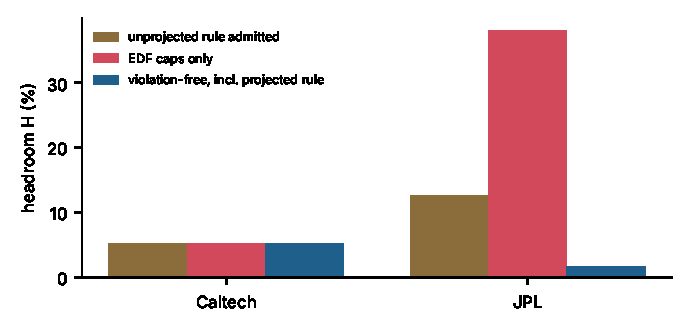
\includegraphics[width=.55\linewidth]{figs/fig_headroom_gating.pdf}\caption{Headroom (SCE stand-in, 20 real weekdays) under three admission rules for the reference.}\label{fig:head}\end{figure}

\textbf{Planning heuristic.} For paired daily differences with standard deviation $\sigma_\Delta$ and mean gain $\mu$, a normal-approximation test needs $N\gtrsim(z_{1-\delta/2}+z_\beta)^2\sigma_\Delta^2/\mu^2$ days. Since $\mu\le HJ_{\rm ref}$ under the programme's model, $N$ grows at least as $H^{-2}$ at fixed $\sigma_\Delta$, so a headroom of a few per cent requires hundreds of days for a significant gain to be resolved.

\subsection{Twin fidelity}\label{sec:res-twin}
For identical random actions the twin and the simulator agree to $3.5\times10^{-16}$ relative cost on 10 synthetic days and $2\times10^{-16}$ on 10 real days, with no violations. Autograd against central differences on 60 non-zero-gradient coordinates has median relative error $3\times10^{-7}$ (synthetic), $1.3\times10^{-4}$ (Caltech) and $1.7\times10^{-6}$ (JPL), with 77, 50 and 67\% of coordinates within $10^{-4}$; the remainder lie at maximum or clip kinks.

\subsection{Restoration, projection and pathwise learning}\label{sec:res-pgd}
\textbf{The effect of the restoration on the same action.} The tuned reference at JPL costs 754.5 under the exact QP and 889.3 under ray scaling, a difference of 17.9\% for an identical proposed action. Replacing the ray scaling of the twin by the averaged projection does not alter the cost of the starting rule in the twin appreciably (1164 against 1140 on six training days), whereas the summed Jacobi form gives 2443. The averaged form is therefore necessary but not sufficient: the improvement over the baseline construction comes from the gradient structure together with the inclusive-boundary clamp.

\textbf{Convergence.} With the Cimmino-averaged projection, the inclusive clamp and the residual policy started at the reference, training moved the twin cost in every one of twelve runs (3 seeds, two sites, two splits). Under the exact QP in the simulator, with no violation in any run, the results are as in Table~\ref{tab:pgd}.
\begin{table}[h]\centering\footnotesize\setlength{\tabcolsep}{3pt}
\begin{tabular}{@{}L{2.5cm}cccccc@{}}\toprule Split & Ref. & LP (nom. / corr.) & Learned (3 seeds) & Change (\%) & 95\% CI, seed 0 & Days better\\\midrule
JPL, random & 754.5 & 748.9 / 738.4 & 718.0, 719.8, 717.6 & $-4.8$, $-4.6$, $-4.9$ & $-51$ to $-21$ & 18, 17, 17\\
JPL, 2019 chron. & 969.1 & 975.6 / 961.8 & 915.8, 919.1, 917.1 & $-5.5$, $-5.2$, $-5.4$ & $-75$ to $-32$ & 17, 16, 17\\
Caltech, random & 386.1 & 362.2 / 354.6 & 379.7, 379.2, 378.9 & $-1.7$, $-1.8$, $-1.9$ & $-14$ to $-1$ & 13, 11, 11\\
Caltech, 2019 chron. & 320.5 & 304.4 / 296.6 & 317.3, 317.4, 316.9 & $-1.0$, $-1.0$, $-1.1$ & $-7$ to $+0.4$ & 12, 10, 13\\\bottomrule
\end{tabular}\caption{Mean cost per day (\$) on 20 held-out days (LP column: perfect-foresight plan executed in the simulator, with nominal and with corrected efficiency), evaluated in the simulator through the exact QP. Pathwise policy with Cimmino projection and residual initialisation; ``Days better'' counts days on which the learned policy is cheaper for each seed. The served-energy fraction at JPL (random split) is 0.924 against 0.921 for the reference.}\label{tab:pgd}\end{table}
\begin{figure}[h]\centering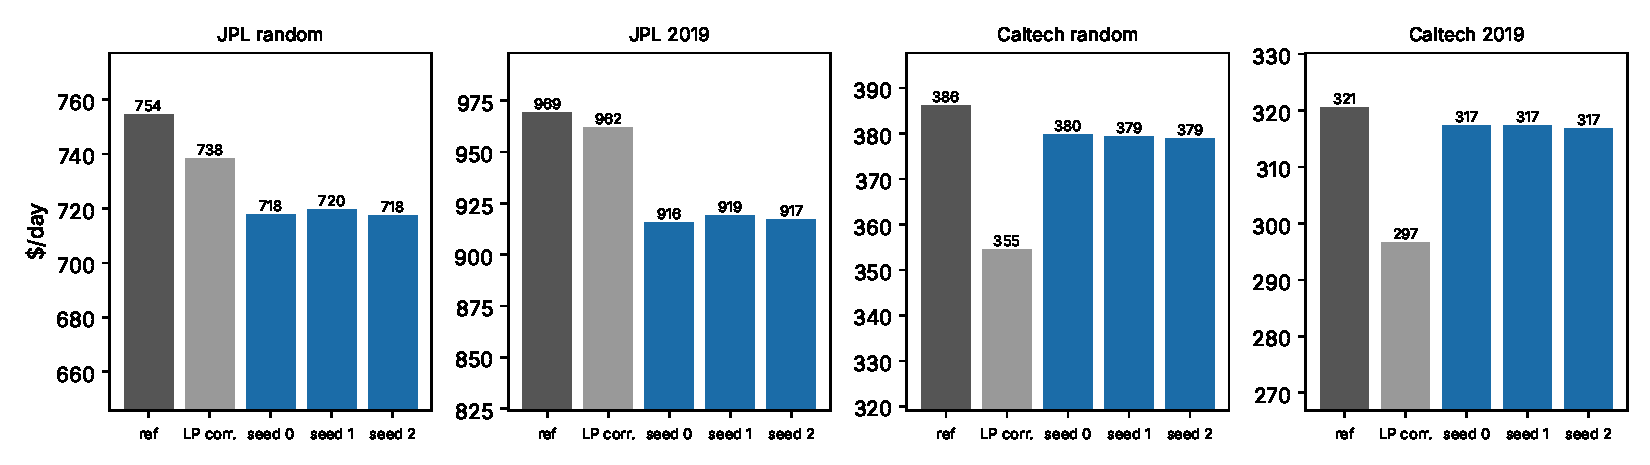
\includegraphics[width=.95\linewidth]{figs/fig_pathwise_closedloop.pdf}\caption{Held-out cost per day under the exact QP: tuned reference, perfect-foresight LP, and three seeds of the pathwise policy.}\label{fig:pw}\end{figure}
At JPL the learned policy is 4.6 to 5.5\% below the reference on both splits, better on 16 to 18 of 20 days, and below the perfect-foresight plan on both splits, including the corrected plan (738.4 and 961.8). A plan executed in the simulator is therefore a reference rather than a bound, because the programme still omits the unmet-energy coupling to the SoC taper and the demand-charge timing; the corrected plan is nevertheless the more accurate of the two. At Caltech the gain, 1.0 to 1.9\%, captures roughly a fifth of the 7.5 to 8.2\% gap to the corrected plan, and the 95\% interval of seed 0 on the chronological split includes zero. We therefore claim a robust gain at JPL and a modest and statistically weaker one at Caltech. With ray-scaling restoration and a full-rate start, by contrast, six of seven JPL runs and all three Caltech chronological runs remained at the starting plateau.

\textbf{Planning versus learning.} On synthetic stress days (headroom 32.7\%) with perfect foresight, open-loop Adam through the twin reaches 795 against 610 for the programme, so plain gradient descent is a weak planner for this piecewise-linear problem; a causal learned policy (781) is better than the 300-iteration planner. The reason is open.

\subsection{Residual world model and the conformal margin}\label{sec:wm}
\textbf{One-step accuracy.} On held-out synthetic days (Table~\ref{tab:wm}), without the physics base the network is about 70 times worse in voltage at every sample size, so the analytic model carries most of the accuracy. The residual halves the branch-flow error and reduces the maximum voltage error by a factor of 2.8 with about a thousand transitions, while the mean voltage error improves by 15\%.
\begin{table}[h]\centering\small
\begin{tabular}{@{}lcccc@{}}\toprule Model & Voltage MAE & Voltage max error & Branch-$S$ MAE & SoC MAE\\\midrule
$F_{\rm base}$ only & $2.1\times10^{-4}$ & $5.5\times10^{-3}$ & $6.4\times10^{-3}$ & 0.024\\
$+N_\theta$, 100 samples & $2.7\times10^{-4}$ & $6.0\times10^{-3}$ & $3.0\times10^{-3}$ & 0.031\\
$+N_\theta$, 2880 samples & $1.8\times10^{-4}$ & $2.0\times10^{-3}$ & $2.1\times10^{-3}$ & 0.048\\
Black-box, 100 samples & $1.5\times10^{-2}$ & 0.16 & 0.046 & 0.14\\
Black-box, 2880 samples & $1.6\times10^{-2}$ & 0.20 & 0.045 & 0.083\\\bottomrule
\end{tabular}\caption{One-step prediction error (p.u. except SoC), mean of three seeds.}\label{tab:wm}\end{table}

\textbf{The SoC error is a boundary effect.} The SoC error of $F_{\rm base}$ (0.024) arises from the 3\% of occupied slots that change occupant within the step; on slots that remain occupied it is $1.1\times10^{-4}$. The residual SoC head, trained mostly on the boundary steps, raises the continuous-slot error to 0.025; removing it restores $1.1\times10^{-4}$, and a per-slot network adds nothing. $N_\theta$ is therefore applied to voltage and flow only.

\textbf{Margins and dispatch cost.} Table~\ref{tab:a5} reports the 1\% margins and, in the last columns, the dispatch cost and the exact-AC violations of the tuned reference executed through the safety layer built with each margin.
\begin{table}[h]\centering\footnotesize\setlength{\tabcolsep}{3pt}
\begin{tabular}{@{}llcccccc@{}}\toprule Data & Margin source & $\tau_v$ (p.u.) & $\tau_S$ (rating) & Cover $v$, $S$ & Dispatch (\$/day) & Viol. days & Served\\\midrule
\multirow{4}{*}{Synthetic} & zero margin & 0 & 0 & -- & 358.3 & 0.50 & 0.999\\
 & $F_{\rm base}$ only & 0.0069 & 0.0228 & 0.997, 0.997 & 365.1 & 0 & 0.998\\
 & $F_{\rm base}+N_\theta$ (grid) & 0.0012 & 0.0030 & 0.990, 0.992 & 362.4 & 0 & 0.998\\
 & black-box & 0.0352 & 0.0864 & 0.997, 0.988 & 1455.2 & 0 & 0.698\\\midrule
\multirow{4}{*}{JPL} & zero margin & 0 & 0 & -- & 677.8 & 0 & 0.858\\
 & $F_{\rm base}$ only & 0.0008 & 0.0165 & 1.000, 0.986 & 682.3 & 0 & 0.854\\
 & $F_{\rm base}+N_\theta$ (grid) & 0.0012 & 0.0047 & 0.982, 0.993 & 678.9 & 0 & 0.857\\
 & black-box & 0.0487 & 0.7652 & 0.973, 0.986 & 1285.7 & 0 & 0.469\\\midrule
\multirow{4}{*}{Caltech} & zero margin & 0 & 0 & -- & 407.8 & 0 & 0.750\\
 & $F_{\rm base}$ only & 0.0004 & 0.0156 & 0.969, 0.970 & 407.8 & 0 & 0.750\\
 & $F_{\rm base}+N_\theta$ (grid) & 0.0011 & 0.0022 & 0.975, 1.000 & 407.8 & 0 & 0.750\\
 & black-box & 0.0613 & 0.5875 & 0.965, 1.000 & 818.1 & 0 & 0.279\\\bottomrule
\end{tabular}\caption{One-step 1\% margins, coverage on the held-out half, and dispatch of the tuned reference through the QP layer on 10 test days. Learned variants are means over three seeds. ``Viol. days'' is the fraction of days with any exact-AC violation.}\label{tab:a5}\end{table}
The grid-only residual reduces the rating-normalised branch margin by 7.6, 3.5 and 7.1 times on synthetic, JPL and Caltech data (and by 9.8 times in the one-step synthetic study at the same level), while retaining a coverage of at least 0.97 on the held-out half. The voltage margin shrinks by 5.7 times on synthetic days but is larger on real transitions (0.0012 against 0.0004 to 0.0008), so the voltage benefit does not transfer. On synthetic days, where the network binds, the residual margin lowers dispatch cost by \$2.7 per day (0.7\%) relative to the physics-only margin with no violations, whereas a zero margin is \$7 cheaper and violates the exact network on half of the days. On the real sites the network rarely binds under the reference, so cost differences are below \$5 per day and the effect of the margin on cost cannot be resolved. The black-box margin is large enough to suppress dispatch (cost two to four times higher, with 28 to 70\% of the energy served).

\subsection{Bidirectional vehicle-to-grid dispatch}\label{sec:v2g}
\textbf{Headroom.} On eight synthetic days the perfect-foresight programme without discharge costs 352.2 and with discharge 275.3, against 380.6 for the best non-discharging reference tuned on 30 training days; the safe rule greedy V2G rule costs 518.7. The clairvoyant headroom against the reference is therefore 27.7\%, of which 20.2 points are attributable to discharge, whereas the causal rule is 36.3\% worse than the reference. On twenty held-out 2019 days of real sessions (stress regime, SCE stand-in price, corrected oracle), discharge is worth almost nothing: the perfect-foresight programme costs 961.3 with and 961.8 without discharge at JPL (reference 972.4), and 296.0 with and 296.6 without at Caltech (reference 320.4), while the safe rule projected greedy V2G rule is 4.0\% (JPL, 1011.2) and 17.5\% (Caltech, 376.5) worse than the reference. The large clairvoyant value of discharge is therefore a property of the synthetic session generator, whose dwell times are long relative to the charging need, and not of the real sessions, in which the energy request consumes most of the available dwell time.

\textbf{Pathwise learning.} The bidirectional twin matches the simulator to within $2\times10^{-4}$ (513.2 against 513.19 on six days), and the gradient is locally exact (a step of $10^{-2}$ along the normalised gradient changes the cost by $-12.2$ against a first-order prediction of $-11.6$). Nevertheless, policies initialised at the reference did not capture the headroom (Table~\ref{tab:v2g}).
\begin{table}[h]\centering\small
\begin{tabular}{L{6.0cm}ccc}\toprule Policy (8 held-out synthetic days) & Cost (\$/day) & vs reference & Violations\\\midrule
Tuned non-discharging reference (EDF cap 1.0) & 380.6 & -- & 0\\
projected greedy V2G rule & 518.7 & $+36.3\%$ & 0\\
Perfect-foresight LP, no discharge & 352.2 & $-7.5\%$ & 0\\
Perfect-foresight LP, with discharge & 275.3 & $-27.7\%$ & 0\\\midrule
Pathwise, backtracking normalised descent, 3 seeds & 381.3, 383.0, 386.9 & $+0.2$, $+0.6$, $+1.7\%$ & 0\\
Pathwise, Adam (five-feature policy), 3 seeds & 409.3, 402.5, 407.7 & $+7.5$, $+5.8$, $+7.1\%$ & $<10^{-3}$\\\bottomrule
\end{tabular}\caption{Bidirectional dispatch on synthetic days, simulator costs through the exact QP. The learned policies start at the reference and do not improve on it; the backtracking variant stops at a point where no tested step decreases the training cost.}\label{tab:v2g}\end{table}
The failure is not attributable to the step size: Adam with learning rates from $10^{-5}$ to $10^{-2}$, backtracking normalised gradient descent, and a reduced five-feature policy gave the outcomes of Table~\ref{tab:v2g}. Among plausible mechanisms are the discontinuity of the discharge indicator in the degradation term, the unmet-energy cliff that couples a discharge decision to a recharge decision many steps later, and the sign structure of the signed action at the zero point. We have not isolated which of these dominates and do not claim that pathwise learning cannot solve the bidirectional problem; we report only that the present construction does not.

\subsection{Critic-based baseline}\label{sec:rl}
On real Caltech days over three seeds, residual SafeTD3 costs $+6.3$, $+4.4$ and $+8.5\%$ relative to the tuned cap at residual scale 0.3 and $+1.8\%$ at 0.1; plain TD3 is $+41\%$. The regret grows with the permitted deviation, there are no violations, and lower exploration noise, tuned hyperparameters or removal of the conformal margin do not change the sign. On the synthetic stress days, where the headroom is 32.7\% and the tuned cap costs 906.7, residual TD3 over three seeds costs 1086.0, 1120.0 and 1068.8 without the model-based term (mean 1091.6, $+20.4\%$) and 1030.2, 1100.6 and 1073.4 with the one-step model-based term $\lambda_{\rm mb}=0.5$ (mean 1068.1, $+17.8\%$). The one-step term lowers the cost on two of three seeds and its mean effect is 2.2\%, which is small relative to the 17.8\% regret. The summed exact-AC violation per day does not exceed $2.5\times10^{-4}$ p.u. in any run. Two pathwise parametrisations are available on the same days and the same exact-QP evaluation. The residual policy with Cimmino projection (this paper's construction) costs 851.8, 860.5 and 850.2, which is 5.1 to 6.2\% below the tuned cap, with no violation and better on 12 to 15 of 20 days. A direct parametrisation, in which the network proposes the action fraction without a reference anchor and restoration is by ray scaling, costs 779.7, 783.2 and 780.9, which is 13.7 to 14.0\% below the cap. Where the headroom is large and the reference is far from the optimum (the tuned cap is 0.3 of capacity), the anchor limits the region reachable within the residual bound $\beta=0.5$, and the direct parametrisation is preferable; where the reference is near the optimum, as in the real-data experiments, the anchor is what allows learning to start. The critic-based policy is 17.8 to 20.4\% worse than the cap in the same setting, and the one-step model-based term does not close the gap that the full-horizon gradient closes. The comparison is not a controlled test of the gradient horizon, because TD3 draws fresh days in every episode whereas the pathwise policies use 30 fixed training days.

%% =====================================================================
\section{Discussion and Limitations}\label{sec:disc}
\textbf{What the analysis explains.} Two causes together account for the inability of the baseline construction to learn: the restoration operator annihilates the gradient along the action scale on binding rows (Proposition~\ref{prop:ray}), and the standard clamp creates a stationary point at the reference (Proposition~\ref{prop:clip}). Each can be corrected without changing the safety guarantee, since the executed action in the simulator still passes through the exact QP. The twin is trained under a restoration that differs from the deployed one, and Table~\ref{tab:pgd} shows that the policies transfer: the cost in the twin under the Cimmino projection and in the simulator under the same projection agree to within 0.7\% (0.01\% in the JPL random split), and the live cost under the exact QP is lower still.

\textbf{Scope.} The network is balanced and single-phase, there is one feeder and two sites, and the chronological split covers one year. The design principle in the introduction is not tested outside this setting. Real-day headroom depends strongly on the oracle correction, and the learned policies capture a minor part of it (1 to 5\% of cost against corrected headroom of 3.5 to 26\%), so a substantial gap to the perfect-foresight plan remains. Three seeds is a small number: the intervals for Caltech include zero in some runs. The world-model results are one-step; the margin reduction is not shown to carry over to multi-step prediction. Bidirectional learning is a negative result. No constraint violation occurred in any evaluated run, which is an empirical observation and not a guarantee; the conformal statements hold under their stated assumptions and for one step.

%% =====================================================================
\section{Conclusion}\label{sec:concl}
We have examined how a polyhedral safety layer interacts with pathwise policy learning on a physical system for which an exact reference is available. The main results are an exact characterisation of why uniform rescaling cannot support gradient-based learning, a Cimmino-averaged projection and an inclusive-boundary clamp that remove the obstruction, and measured improvements over a tuned violation-free reference of 4.6 to 5.5\% at JPL (twelve of twelve runs converge, no AC violations on two splits) and 1.0 to 1.9\% at Caltech, where the headroom is smaller. On the safety side, a margin fixed at one load level does not survive load shift, adaptive conformal inference does, the required margin grows with the square of the load for a physical reason, and a joint margin is needed for joint coverage. A physics-based world model with a grid-only learned residual shrinks the branch margin by 3.5 to 9.8 times, with a measurable but modest effect on dispatch cost where the network binds. The architecture, which couples an analytic base model with a calibrated residual, an unrolled projection and a residual policy, is stated in a form that does not depend on the power-systems instance, and the natural next tests are a three-phase unbalanced feeder, multi-step calibration of the residual margin, a restoration with an exact differentiable projection, and a treatment of the bidirectional problem in which the discharge decision is decoupled from the recharge decision.

\paragraph{Reproducibility.} Code, result files and a SHA-256 manifest accompany the paper (\texttt{REPRODUCE.md}). Versions are pinned, and tests cover twin fidelity, gradients, the QP layer and the conformal procedures. Figures are generated from stored result files.

%% =====================================================================
\newpage
\section*{References}
\footnotesize\setlength{\itemsep}{2pt}
\begin{list}{}{\setlength{\leftmargin}{2.4em}\setlength{\labelwidth}{2.4em}\setlength{\itemsep}{2pt}\setlength{\parsep}{0pt}}
\item[\textbf{[1]}] S. Orfanoudakis, C. Diaz-Londono, Y. E. Yilmaz, P. Palensky, P. P. Vergara, EV2Gym: a flexible V2G simulator for EV smart charging research and benchmarking, IEEE Trans. Intell. Transp. Syst. 26(2), 2025.
\item[\textbf{[2]}] S. Orfanoudakis, F. A. Oliehoek, P. Palensky, P. P. Vergara, Physics-informed reinforcement learning for large-scale EV smart charging considering distribution network voltage constraints, arXiv:2510.12335.
\item[\textbf{[3]}] C. Huang, J. Fan, W. Wang, H. Wang, Safe decentralized operation of EV virtual power plant with limited network visibility via multi-agent reinforcement learning, arXiv:2604.03278.
\item[\textbf{[4]}] J. Ruddick, G. Ceusters, G. Van Kriekinge, E. Genov, C. De Cauwer, T. Coosemans, M. Messagie, Real-world validation of safe reinforcement learning, model predictive control and decision tree-based home energy management systems, arXiv:2408.07435.
\item[\textbf{[5]}] Z. J. Lee, T. Li, S. H. Low, ACN-Data: analysis and applications of an open EV charging dataset, ACM e-Energy, 2019.
\item[\textbf{[6]}] Z. J. Lee, D. Johansson, S. H. Low, ACN-Sim: an open-source simulator for data-driven electric vehicle charging research, IEEE SmartGridComm, 2019.
\item[\textbf{[7]}] D. Millstein, E. O'Shaughnessy, R. Wiser, Wholesale Electricity Prices tool, Lawrence Berkeley National Laboratory.
\item[\textbf{[8]}] M. E. Baran, F. F. Wu, Network reconfiguration in distribution systems for loss reduction and load balancing, IEEE Trans. Power Delivery 4(2), 1989.
\item[\textbf{[9]}] M. Farivar, S. H. Low, Branch flow model: relaxations and convexification, IEEE Trans. Power Systems 28(3), 2013.
\item[\textbf{[10]}] B. Amos, J. Z. Kolter, OptNet: differentiable optimization as a layer in neural networks, ICML 2017.
\item[\textbf{[11]}] A. Agrawal, B. Amos, S. Barratt, S. Boyd, S. Diamond, J. Z. Kolter, Differentiable convex optimization layers, NeurIPS 2019.
\item[\textbf{[12]}] G. Dalal, K. Dvijotham, M. Vecerik, T. Hester, C. Paduraru, Y. Tassa, Safe exploration in continuous action spaces, arXiv:1801.08757, 2018.
\item[\textbf{[13]}] K. P. Wabersich, M. N. Zeilinger, A predictive safety filter for learning-based control of constrained nonlinear dynamical systems, Automatica 129, 2021.
\item[\textbf{[14]}] J. Garc\'ia, F. Fern\'andez, A comprehensive survey on safe reinforcement learning, J. Mach. Learn. Res. 16, 2015.
\item[\textbf{[15]}] J. Achiam, D. Held, A. Tamar, P. Abbeel, Constrained policy optimization, ICML 2017.
\item[\textbf{[16]}] S. Fujimoto, H. van Hoof, D. Meger, Addressing function approximation error in actor-critic methods, ICML 2018.
\item[\textbf{[17]}] T. Johannink et al., Residual reinforcement learning for robot control, IEEE ICRA, 2019.
\item[\textbf{[18]}] T. Silver, K. Allen, J. Tenenbaum, L. Kaelbling, Residual policy learning, arXiv:1812.06298, 2018.
\item[\textbf{[19]}] A. Y. Ng, D. Harada, S. Russell, Policy invariance under reward transformations: theory and application to reward shaping, ICML 1999.
\item[\textbf{[20]}] V. Vovk, A. Gammerman, G. Shafer, Algorithmic Learning in a Random World, Springer, 2005.
\item[\textbf{[21]}] J. Lei, M. G'Sell, A. Rinaldo, R. J. Tibshirani, L. Wasserman, Distribution-free predictive inference for regression, J. Am. Stat. Assoc. 113(523), 2018.
\item[\textbf{[22]}] A. N. Angelopoulos, S. Bates, Conformal prediction: a gentle introduction, Found. Trends Mach. Learn. 16(4), 2023.
\item[\textbf{[23]}] I. Gibbs, E. J. Cand\`es, Adaptive conformal inference under distribution shift, NeurIPS 2021.
\item[\textbf{[24]}] S. Huriot, I. Tabbara, H. Sibai, Safe control using learned safety filters and adaptive conformal inference, arXiv:2604.18482.
\item[\textbf{[25]}] D. Fern\'andez-Zapico, T. Hofman, M. Salazar, Stochastic model predictive control of charging energy hubs with conformal prediction, arXiv:2504.00685.
\item[\textbf{[26]}] N. Heess, G. Wayne, D. Silver, T. Lillicrap, T. Erez, Y. Tassa, Learning continuous control policies by stochastic value gradients, NeurIPS 2015.
\item[\textbf{[27]}] J. Xu, V. Makoviychuk, Y. Narang, F. Ramos, W. Matusik, A. Garg, M. Macklin, Accelerated policy learning with parallel differentiable simulation, ICLR 2022.
\item[\textbf{[28]}] H. J. T. Suh, M. Simchowitz, K. Zhang, R. Tedrake, Do differentiable simulators give better policy gradients? ICML 2022.
\item[\textbf{[29]}] L. Metz, C. D. Freeman, S. S. Schoenholz, T. Kachman, Gradients are not all you need, arXiv:2111.05803, 2021.
\item[\textbf{[30]}] C. D. Freeman et al., Brax: a differentiable physics engine for large scale rigid body simulation, NeurIPS Datasets and Benchmarks, 2021.
\item[\textbf{[31]}] Y. Hu et al., DiffTaichi: differentiable programming for physical simulation, ICLR 2020.
\item[\textbf{[32]}] M. \"Oz, J. H\"orter, K. Phipps, C. Debus, A. Streit, M. G\"otz, Differentiable power-flow optimization, arXiv:2603.28203.
\item[\textbf{[33]}] G. Cimmino, Calcolo approssimato per le soluzioni dei sistemi di equazioni lineari, La Ricerca Scientifica 9(2), 1938.
\item[\textbf{[34]}] Y. Censor, T. Elfving, G. T. Herman, T. Nikazad, On diagonally relaxed orthogonal projection methods, SIAM J. Sci. Comput. 30(1), 2008.
\item[\textbf{[35]}] P. Henderson, R. Islam, P. Bachman, J. Pineau, D. Precup, D. Meger, Deep reinforcement learning that matters, AAAI 2018.
\item[\textbf{[36]}] R. Agarwal, M. Schwarzer, P. S. Castro, A. Courville, M. G. Bellemare, Deep reinforcement learning at the edge of the statistical precipice, NeurIPS 2021.
\item[\textbf{[37]}] J. R. V\'azquez-Canteli, Z. Nagy, Reinforcement learning for demand response: a review of algorithms and modeling techniques, Applied Energy 235, 2019.
\end{list}
\end{document}
